% trilemma.tex — The Attribution Impossibility trilemma figure
% Compiles standalone:  cd paper/figures && pdflatex trilemma.tex
% Include in paper:     
\includegraphics[width=\textwidth]{figures/trilemma.pdf}
%
\documentclass[border=8pt]{standalone}

\usepackage{tikz}
\usepackage{amsmath,amssymb}
\usepackage{xcolor}

\usetikzlibrary{positioning, arrows.meta, calc, decorations.pathreplacing}

\definecolor{familyA}{RGB}{230,120,30}   % orange
\definecolor{familyB}{RGB}{40,100,200}   % blue
\definecolor{impossiblered}{RGB}{200,30,30}
\definecolor{bardark}{RGB}{60,60,60}
\definecolor{barlight}{RGB}{160,160,160}
\definecolor{dashgreen}{RGB}{50,150,80}
\definecolor{trivia}{RGB}{140,140,140}

\begin{document}
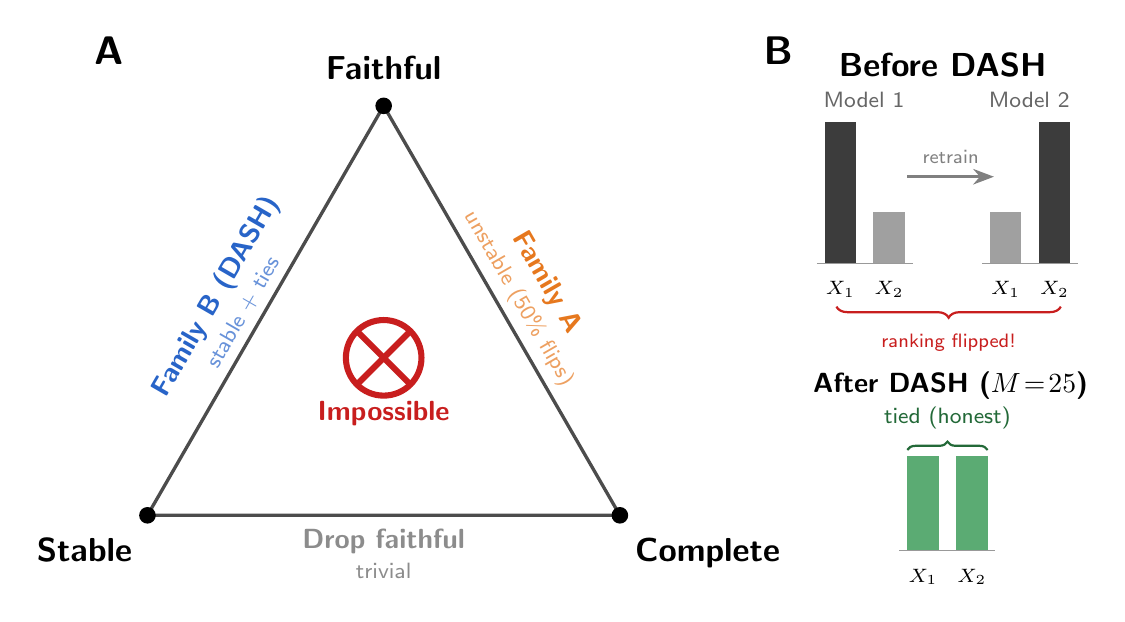
\begin{tikzpicture}[
    every node/.style={font=\sffamily},
    >=Stealth
  ]

  % ============================================================
  %  PANEL A — Trilemma Triangle
  % ============================================================
  \begin{scope}[shift={(0,0)}]

    % Equilateral triangle
    \coordinate (F) at (0, 5.2);       % top: Faithful
    \coordinate (S) at (-3.0, 0);      % bottom-left: Stable
    \coordinate (C) at (3.0, 0);       % bottom-right: Complete

    % Draw edges
    \draw[line width=1.2pt, black!70] (F) -- (S) -- (C) -- cycle;

    % Vertex labels
    \node[above=6pt of F, font=\sffamily\bfseries\large] {Faithful};
    \node[below left=5pt and 2pt of S, font=\sffamily\bfseries\large] {Stable};
    \node[below right=5pt and 2pt of C, font=\sffamily\bfseries\large] {Complete};

    % Vertex dots
    \fill (F) circle (3pt);
    \fill (S) circle (3pt);
    \fill (C) circle (3pt);

    % --- Central "Impossible" marker (raised for visual centering) ---
    \coordinate (center) at (0, 2.0);

    % Red circle with X
    \draw[impossiblered, line width=2.2pt] (center) circle (0.48);
    \draw[impossiblered, line width=2.2pt]
      ($(center)+(-0.33,-0.33)$) -- ($(center)+(0.33,0.33)$);
    \draw[impossiblered, line width=2.2pt]
      ($(center)+(-0.33,0.33)$) -- ($(center)+(0.33,-0.33)$);

    % "Impossible" text
    \node[below=12pt of center, font=\sffamily\bfseries,
          text=impossiblered] {Impossible};

    % --- Edge annotations: single two-line nodes, centered on edge midpoints ---

    % Left edge: Family B (DASH) — at exact midpoint
    \node[rotate=60, anchor=east, align=center,
          text=familyB]
      at ($(F)!0.25!(S) + (-0.45,0.15)$)
      {{\bfseries Family B (DASH)}\\[-1pt]
       {\footnotesize\color{familyB!70} stable $+$ ties}};

    % Right edge: Family A — at exact midpoint
    \node[rotate=-60, anchor=west, align=center,
          text=familyA]
      at ($(F)!0.25!(C) + (0.45,0.15)$)
      {{\bfseries Family A}\\[-1pt]
       {\footnotesize\color{familyA!70} unstable (50\% flips)}};

    % Bottom edge: Drop faithful
    \node[anchor=north, align=center,
          text=trivia]
      at ($(S)!0.5!(C) + (0,-0.05)$)
      {{\bfseries Drop faithful}\\[-1pt]
       {\footnotesize trivial}};

    % Panel label
    \node[anchor=north west, font=\sffamily\bfseries\Large]
      at (-3.8, 6.2) {\textsf{A}};

  \end{scope}

  % ============================================================
  %  PANEL B — Before / After DASH
  % ============================================================
  \begin{scope}[shift={(7.0, -0.3)}]

    \newcommand{\barwidth}{0.4}
    \newcommand{\gapwidth}{0.22}

    % Panel label
    \node[anchor=north west, font=\sffamily\bfseries\Large]
      at (-2.3, 6.5) {\textsf{B}};

    % ----------------------------------------------------------
    %  Top sub-panel: Before DASH
    % ----------------------------------------------------------
    \node[anchor=south, font=\sffamily\bfseries\large]
      at (0.1, 5.75) {Before DASH};

    % Model 1 (left bar chart) — lowered for gap below title
    \begin{scope}[shift={(-1.4, 3.5)}]
      \node[anchor=south, font=\sffamily\footnotesize, text=black!60]
        at (0.5, 1.85) {Model 1};

      \fill[bardark] (0, 0) rectangle (\barwidth, 1.8);
      \node[below=3pt, font=\sffamily\scriptsize] at (\barwidth/2, 0) {$X_1$};

      \fill[barlight] (\barwidth+\gapwidth, 0)
        rectangle (2*\barwidth+\gapwidth, 0.65);
      \node[below=3pt, font=\sffamily\scriptsize]
        at (\barwidth+\gapwidth+\barwidth/2, 0) {$X_2$};

      \draw[black!40] (-0.1, 0) -- (2*\barwidth+\gapwidth+0.1, 0);
    \end{scope}

    % "retrain" arrow — centered between Model 1 right edge and Model 2 left edge
    \draw[->, line width=1pt, black!50]
      (-0.35, 4.6) -- (0.75, 4.6)
      node[midway, above=1pt, font=\sffamily\scriptsize, text=black!50] {retrain};

    % Model 2 (right bar chart) — reversed, same lowered position
    \begin{scope}[shift={(0.7, 3.5)}]
      \node[anchor=south, font=\sffamily\footnotesize, text=black!60]
        at (0.5, 1.85) {Model 2};

      \fill[barlight] (0, 0) rectangle (\barwidth, 0.65);
      \node[below=3pt, font=\sffamily\scriptsize] at (\barwidth/2, 0) {$X_1$};

      \fill[bardark] (\barwidth+\gapwidth, 0)
        rectangle (2*\barwidth+\gapwidth, 1.8);
      \node[below=3pt, font=\sffamily\scriptsize]
        at (\barwidth+\gapwidth+\barwidth/2, 0) {$X_2$};

      \draw[black!40] (-0.1, 0) -- (2*\barwidth+\gapwidth+0.1, 0);
    \end{scope}

    % Red brace: ranking flipped — adjusted to match lowered bars
    \draw[impossiblered, thick, decorate,
          decoration={brace, amplitude=4pt, mirror}]
      (-1.25, 2.95) -- (1.60, 2.95)
      node[midway, below=6pt, font=\sffamily\scriptsize,
           text=impossiblered] {ranking flipped!};

    % ----------------------------------------------------------
    %  Bottom sub-panel: After DASH (M=25) — raised for balance
    % ----------------------------------------------------------
    \node[anchor=south, font=\sffamily\bfseries]
      at (0.2, 1.65) {After DASH ($M\!=\!25$)};

    % Single bar chart — tied
    \begin{scope}[shift={(-0.35, -0.15)}]
      \fill[dashgreen!80] (0, 0) rectangle (\barwidth, 1.2);
      \node[below=3pt, font=\sffamily\scriptsize] at (\barwidth/2, 0) {$X_1$};

      \fill[dashgreen!80] (\barwidth+\gapwidth, 0)
        rectangle (2*\barwidth+\gapwidth, 1.2);
      \node[below=3pt, font=\sffamily\scriptsize]
        at (\barwidth+\gapwidth+\barwidth/2, 0) {$X_2$};

      \draw[black!40] (-0.1, 0) -- (2*\barwidth+\gapwidth+0.1, 0);

      % Tie bracket with label
      \draw[dashgreen!70!black, thick, decorate,
            decoration={brace, amplitude=3pt}]
        (0, 1.28) -- (2*\barwidth+\gapwidth, 1.28)
        node[midway, above=4pt, font=\sffamily\footnotesize,
             text=dashgreen!70!black] {tied (honest)};
    \end{scope}

  \end{scope}

\end{tikzpicture}
\end{document}
